% This is LLNCS.DEM the demonstration file of
% the LaTeX macro package from Springer-Verlag
% for Lecture Notes in Computer Science,
% version 2.4 for LaTeX2e as of 16. April 2010
%
\documentclass{llncs}
%
%\usepackage{makeidx}  % allows for indexgeneration
\usepackage{wrapfig}
\usepackage{array}
\usepackage{float}
\usepackage[english]{babel}
\usepackage{lipsum}
\usepackage{caption}
\usepackage{subcaption}
\usepackage{graphicx}
	\graphicspath{{images/}} 
%\usepackage{cite}
\usepackage[linesnumbered,ruled]{algorithm2e}
\usepackage{courier}
\usepackage{hyperref}
    \hypersetup{colorlinks=true,allcolors=blue}
\usepackage{listings}
	\lstset{
  		basicstyle=\ttfamily,
  		frame=none, 
  		breaklines=true,
  		numbers=left,
  		xleftmargin=2.5em,
  		framexleftmargin=0em,
    	emphstyle=\textbf,
    	float=t
	}
	\lstdefinestyle{ocl}{
  		emph={
        	context, inv
    	}
	}
	\lstdefinestyle{cbp}{
	    basicstyle=\ttfamily\scriptsize,
  		emph={
        	session, create, of, type,
        	set, to, add, hire
    	}
	}
	\lstdefinestyle{xmi}{
		basicstyle=\ttfamily\scriptsize,
  		emph={
        	Node, children
    	}
	}
	\lstdefinestyle{xml}{
	    basicstyle=\ttfamily\scriptsize,
  		emph={
        	register, create, add, to, resource,
        	from, eattribute, remove, ereference,
        	set, unset, session, Roy, Jen,
        	Moss, Richmond
    	}
	}
	\lstdefinestyle{java}{
	    basicstyle=\ttfamily\scriptsize,
  		emph={
        	case, UNSET,
        	instanceof, else, if, void,
        	new, UnsetEAttributeEvent,
        	UnsetEReferenceEvent,
        	@override, public, class, extends
    	}
	}
	\lstdefinestyle{eol}{
	    basicstyle=\ttfamily\scriptsize,
  		emph={
        	var, new, for, in, create, set, of, with, 
        	unset, to, add, remove, delete, register, move,
        	from, position, from, move-within, session, \.
    	}
	}

\begin{document}
\renewcommand{\thelstlisting}{\arabic{lstlisting}}
\renewcommand{\labelitemi}{$\bullet$}
\newcommand{\dk}[1]{\textbf{[DK: #1]}}

\title{An Efficient Loading \\ of Change-Based Models}
%
%\titlerunning{Change-based Persistence and Its Loading Optimisation}  % abbreviated title (for running head)
%                                     also used for the TOC unless
%                                     \toctitle is used
%
\author{
    Anonym%Alfa Yohannis \and Horacio Hoyos Rodriguez \and Fiona Polack \and Dimitris Kolovos
}
%
\authorrunning{
    Anonym%Alfa Yohannis et al.
} % abbreviated author list (for running head)
%
%%%% list of authors for the TOC (use if author list has to be modified)
%\tocauthor{Alfa Yohannis,Horacio Hoyos Rodriguez, Fiona Polack, Dimitris Kolovos}
%

\institute{anonym}
%\institute{Department of Computer Science, University of York, United Kingdom\\
%\email{\{ary506, horacio.hoyos, dimitris.kolovos, fiona.polack\}@york.ac.uk}}

\maketitle              % typeset the title of the contribution
%The first states the problem. The second states why the problem is a problem. The third is my startling sentence. The fourth states the implication of my startling sentence.
\begin{abstract}

Recent work proposed a language-independent change-based persistence (CBP) approach for models conforming to object-oriented metamodelling architectures such as MOF and EMF. In this approach, instead of persisting the state of a model, its full editing history is persisted, and the state of the model is reconstructed at loading time by replaying this history. Storing the entire editing history can be beneficial for precise change detection -- and hence e.g. model merging, incremental execution of model management programs -- but comes at the cost of larger and ever-growing model files and slower loading. In this paper, we contribute a more efficient approach for loading models stored in a change-based format. The proposed approach identifies and skips changes that are superseded by latter changes -- and which therefore have no impact on the eventual state of the model. We evaluate the performance of the new loading approach experimentally and we assess the impact it has on saving change-based models. Our results show that the proposed approach can reduce loading times more than 36\% compared to the baseline CBP loading approach, with a negligible impact on saving.

\end{abstract}

\section{Introduction}
\label{sec:introduction}
Existing approaches for file-based model persistence in metamodelling architectures such as MOF and EMF are predominately state-based.
In such approaches, model files contain snapshots of the models' contents, and activities like version control and change detection are left to external systems such as file-based version-control systems and model differencing facilities.
Activities such as model comparison and change detection are computationally consuming for state-based models and can become a burden when larger models are developed in a collaborative setting. 

In contrast to persisting the \emph{state} of models, the authors of \cite{yohannis2017turning} proposed a change-based approach that persists the full sequence of \emph{changes} made to models instead.
The change-based approach comes with a number of envisioned benefits over stated-based persistence, such as the ability to detect changes much faster and more precisely, which can then have positive knock-on effects on helping developers to diff/merge models in collaborative modelling environments, as well as on facilitating faster incremental model validation and transformation\,\cite{rath2012derived,ogunyomi2015property}.
However, change-based persistence comes at the cost of larger and ever-growing model files, and increased model loading time since all recorded changes need to be replayed to reconstruct a model's state\,\cite{yohannis2017turning}.   

Our work extends the change-based persistence (CBP) approach introduced in \cite{yohannis2017turning}, and proposes and evaluates an approach that reduces loading time of change-based models by avoiding replaying changes that have no impact on the eventual state of the model (e.g. that are superseded by subsequent changes).

The rest of the paper is structured as follows. Section \ref{sec:case_study} introduces a running example and provides a brief overview of the original change-based model persistence approach.
Section \ref{sec:loading_time_optimisation} presents an approach that intends to speed up loading of change-based models, and its supporting data structures. Sect. \ref{sec:complexity_analysis} discuss the time complexity of our approach. Sect. \ref{sec:performance_evaluation} discusses the results of evaluation experiments for assessing the benefits of the proposed approach. Section \ref{sec:related_work} provides an overview of related work, an Sect. \ref{sec:conclusions} concludes this paper and discusses directions for future work.

\section{Running Example}
\label{sec:case_study}
To explain change-based model persistence and the contribution of this work, we use the minimal tree metamodel (expressed in the Eclipse Modelling Framework's Ecore metamodelling language) and model illustrated in Figures \ref{fig:tree_metamodel} and \ref{fig:initial_model}.
We chose EMF/Ecore as the de-facto standard for object-oriented metamodelling, and this contrived example to avoid unnecessary repetition in our discussion, while providing a reasonable coverage of the core features of Ecore (classes, single/multi-valued features, references and attributes).
In this example, tree models consist of named nodes which can -- optionally -- contain other nodes (\emph{children} reference).

\begin{figure}[ht]
    \begin{subfigure}[t]{0.4\linewidth}
        \centering
        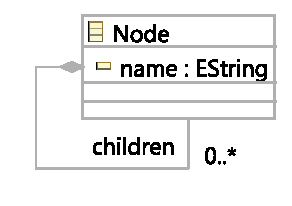
\includegraphics[width=0.8\linewidth]{node_metamodel}
        \caption{The tree metamodel.}
        \label{fig:tree_metamodel}
    \end{subfigure}
    \hfill
    \begin{subfigure}[t]{0.6\linewidth}
        \centering
        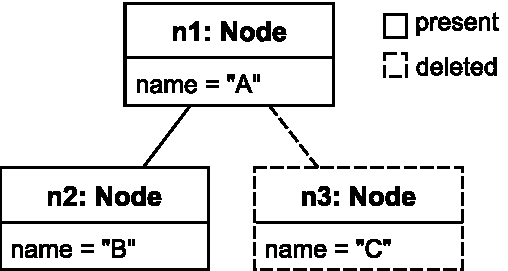
\includegraphics[width=0.6\linewidth]{initial_chart}
        \caption{A model that conforms to the tree metamodel (n3 was created and then deleted)}
        \label{fig:initial_model}
    \end{subfigure}
    \caption{A tree metamodel and its model as the running example.}
    \label{fig:append_speed}
\end{figure}

The model in Fig. \ref{fig:initial_model} consists of two nodes \emph{n1}, \emph{n2}.
To construct this model, we started by creating and naming three nodes (\emph{n1}, \emph{n2} and \emph{n3}).
Nodes \emph{n2} and \emph{n3} were then added as children of \emph{n1}.
Finally, node \emph{n3} was deleted from the model.
The final state of the model is presented in a simplified (state-based) XMI representation in Listing \ref{lst:xmimodel}.

\noindent
\begin{minipage}[t]{0.5\linewidth}
\begin{lstlisting}[style=xmi,caption={State-based representation of the tree model in (simplified) XMI.},label=lst:xmimodel]
<Node id="n1" name="A">
  <children id="n2" name="B"/>
</Node>
\end{lstlisting}
\end{minipage}
\hfill
\begin{minipage}[t]{0.5\linewidth}
\begin{lstlisting}[style=eol,caption={Change-based representation of the tree model.},label=lst:cbpmodel]
create n1 of Node
set n1.name to "A"      
create n2 of Node
set n2.name to "B"      
create n3 of Node
set n3.name to "C"      
add n2 to n1.children   
add n3 to n1.children
remove n3 from n1.children   
delete n3
\end{lstlisting}
\end{minipage}

In contrast to the state-based representation, a CBP representation of the model is illustrated in Listing \ref{lst:cbpmodel} (the syntax is a simplified version of the one introduced in\,\cite{yohannis2017turning}).
Lines 1-6 record the creation and naming of the three nodes, lines 7 and 8 record the addition of \emph{n2} and \emph{n3} as children of \emph{n1} and lines 9-10 capture the deletion of \emph{n3} (while the 'remove' event only represents the removal of an element from its container, the 'delete' event completely removes an element from its model -- cannot be used again).

% Instead of treating the model as a state based, we records all events generated by the the consecutive  operations and persist them into a CBP representation (Listing \ref{lst:cbpmodel}), which contains at least as much information as the state-based representation. Replaying all these events produces the same state as the one captured in the Listing \ref{lst:xmimodel}.  

For small changes made to large models, this approach can be beneficial since we only need to persist the change events every time -- as opposed to the entire model.
However, loading the model by naively replaying all the events is not optimal particularly for models with long editing histories where prior events are often superseded by subsequent events. For example, creating \emph{n3} in line 5, naming it in line 6, and adding it to the children of \emph{n1} in line 8 are cancelled by the subsequent deletion of \emph{n3} in line 10. As such, the events in lines 5, 6, 8, 9 and 10 could be ignored during the loading process without affecting the eventual state of the model.

%An optimisation can be performed by ignoring the superseded events. For example, the deletion of node \emph{n3} makes events (Listing \ref{lst:xmimodel}, lines 5-6, 8-10) related to the node superseded to be replayed. 

\section{Towards Efficient Loading of Change-Based Models}
\label{sec:loading_time_optimisation}
The flowchart in Fig. \ref{fig:flowchart} provides an overview of the editing lifecycle of a CBP model, and the artefacts and data structures involved in it. It also highlights (starred blocks) the extensions proposed compared to the original CBP approach in \cite{yohannis2017turning}.

In the original CBP approach, a model editing session involves three activities: loading a model, editing it, and saving new changes back to the model file\footnote{After saving a model, the user can make further changes and save it again.}. Loading is achieved by reading and replaying a sequence of change events stored in a CBP-formatted file. During the editing process, changes to the model are stored in a memory-based data structure (``Change events''), which are serialised and appended at the end of the CBP-formatted model file, and then flushed from memory, every time the model is saved.

Bare in mind that one principle underlies the use of change-based approach is to persist every change made to a model and therefore no single relevant events should be removed from being persisted. Thus, compression -- the removal of superseded events -- before saving a model is undesired and avoided in order to preserve the whole history of a model as it is. Therefore, the proposed approach adds two new artefacts: a ``Model History'' data structure which is populated with change events and which is used to detect superseded events prior to saving, and an ``Ignore Set'' file for each CBP model, which persists the position (i.e. line numbers) of superseded events so that they can be ignored the next time the model is loaded. 

\begin{figure}[ht]
\centering
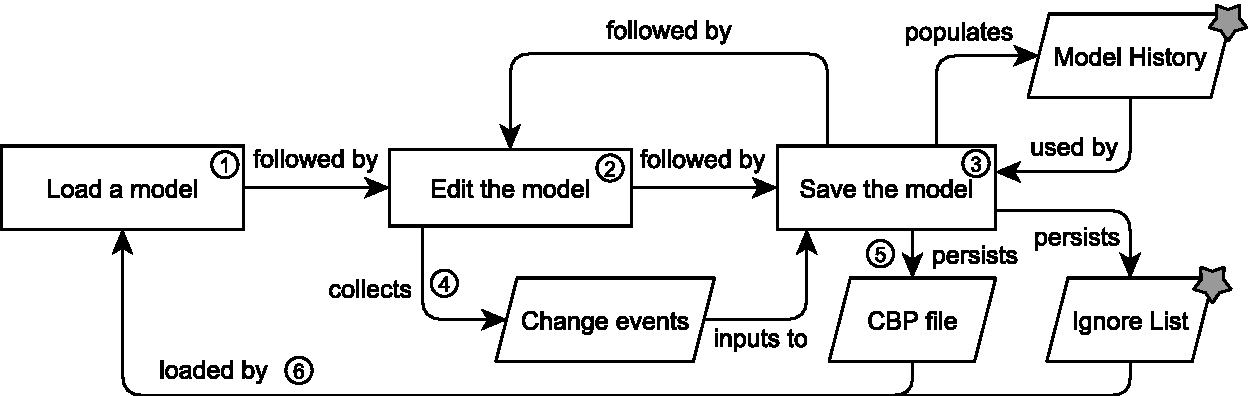
\includegraphics[width=\linewidth]{flowchart}
\caption{The context flowchart of optimising loading performance of CBP.}
\label{fig:flowchart}
\end{figure}

\subsection{Model History}
\label{subsec:model_history}
The proposed approach uses a data structure that memorises elements' events and their position (line number) in a CBP representation so it can reason about the events of a particular element and determine which of them are superseded.
For the rest of the discussion the line number in the CBP representation is referred to as the \emph{event number}.
The proposed data structure is presented in Fig. \ref{fig:object_history} as a class diagram.  

\begin{figure}[ht]
\centering
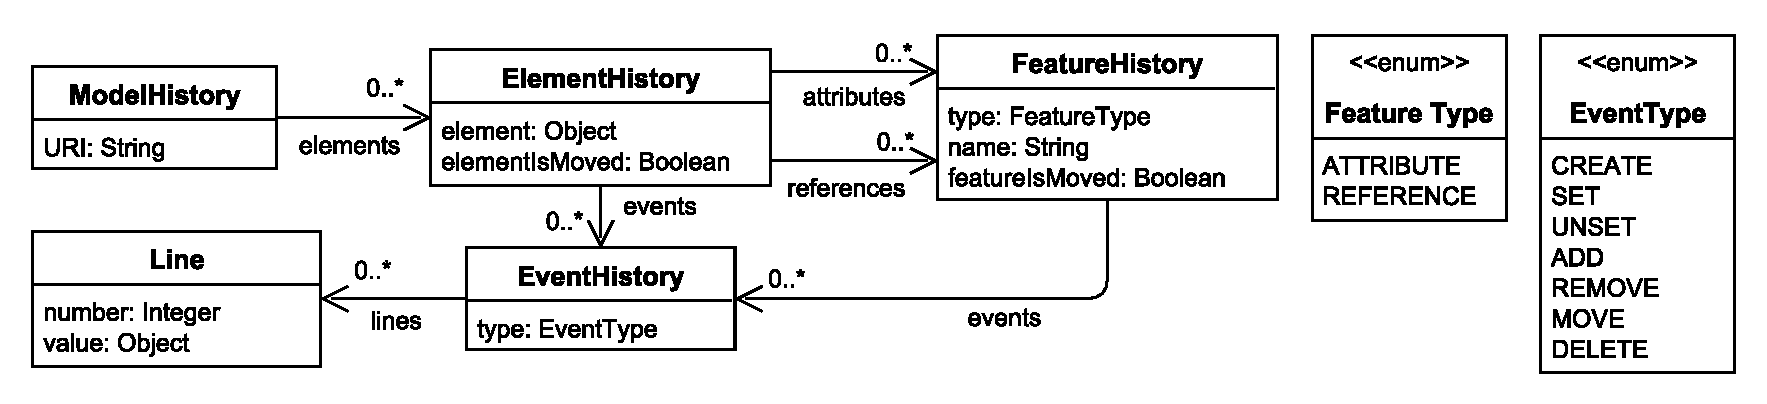
\includegraphics[width=\linewidth]{object_history}
\caption{The class diagram of Model History.}
\label{fig:object_history}
\end{figure}

A \emph{ModelHistory} has a \emph{URI} attribute to identify the model for which it records changes and can have many \emph{ElementHistory} elements.
An \emph{ElementHistory} has an \emph{element} field that identifies the element that it refers to. 
Every \emph{ElementHistory} can have many \emph{FeatureHistories} to represent the editing histories of individual features (i.e. references/attributes) of the element. 
A \emph{FeatureHistory} has three fields: \emph{type} to identify the feature's type (attribute or reference) and \emph{name} to identify the feature's name.

\begin{figure}[ht]
    \centering
    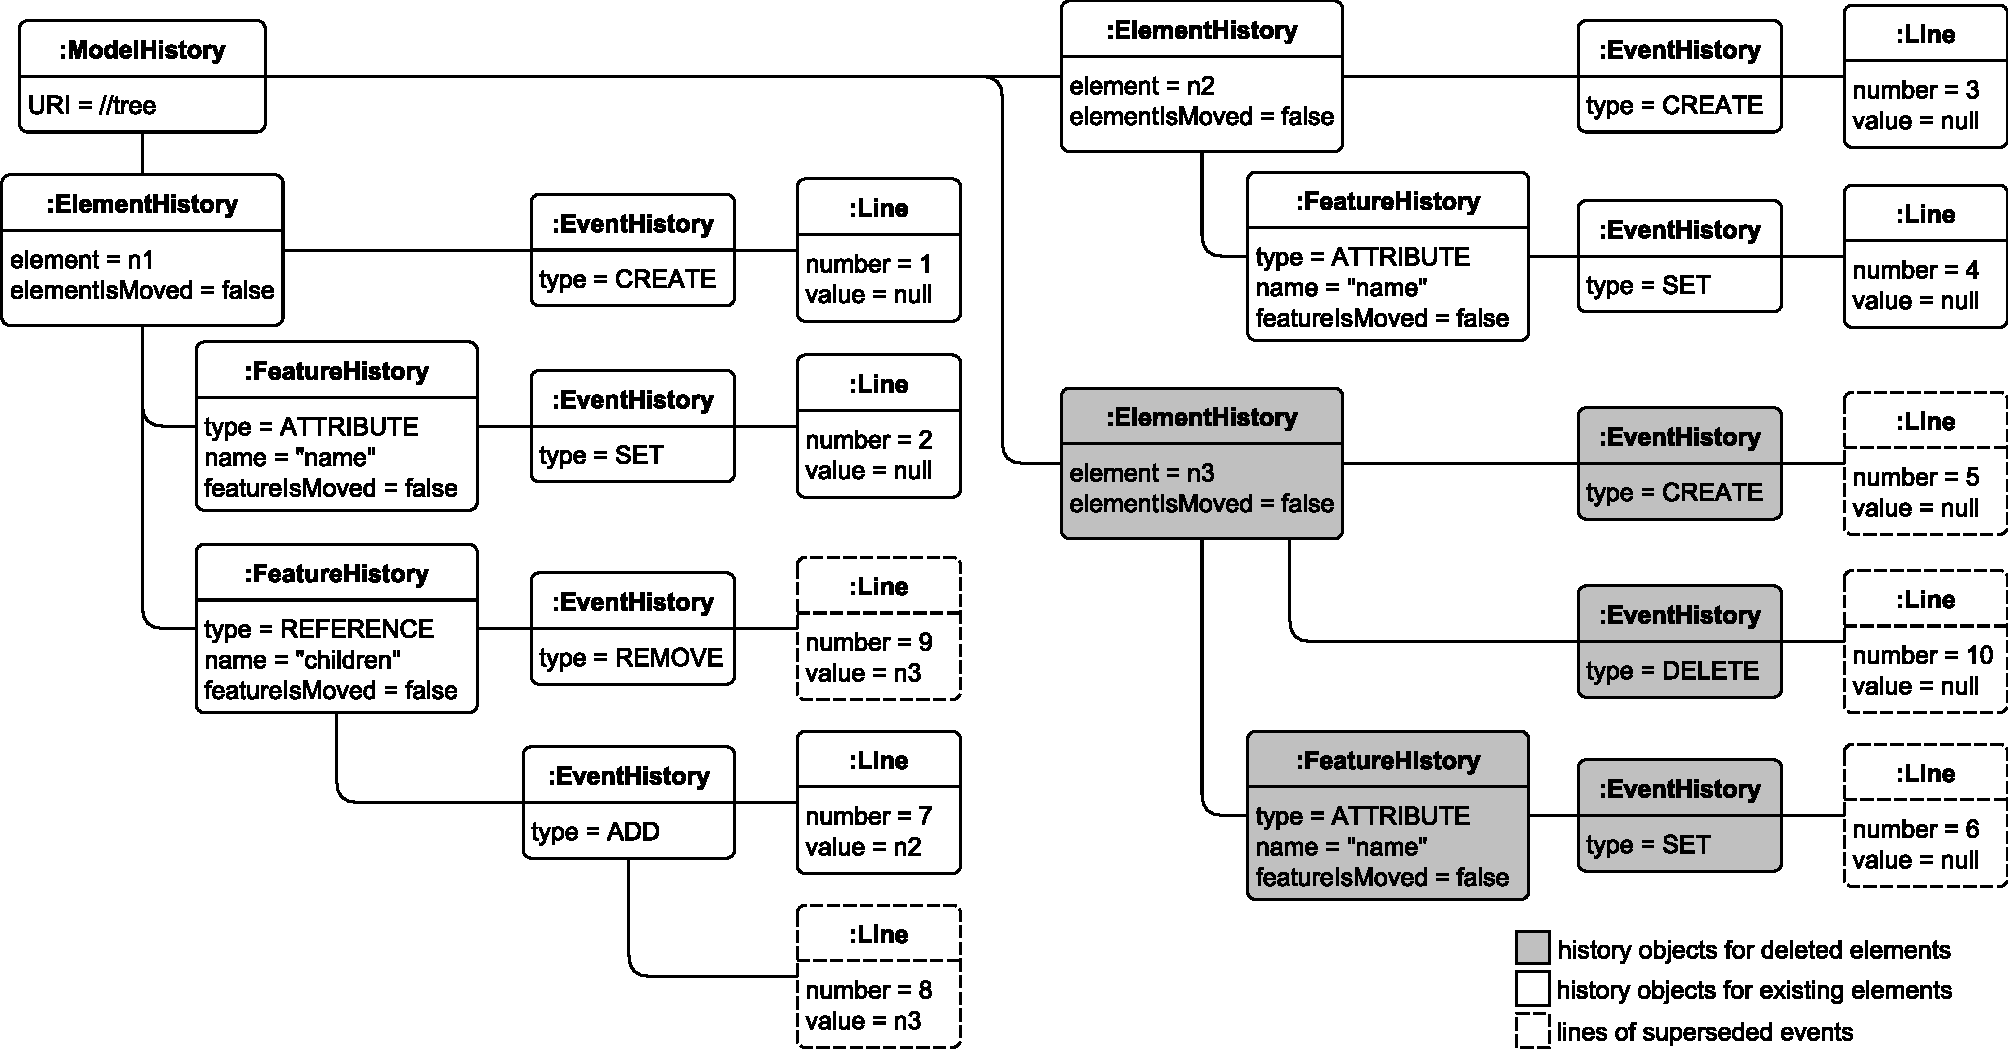
\includegraphics[width=\linewidth]{history_structure}
    \caption{The object diagram of the model history of the CBP model in Listing \ref{lst:cbpmodel}.}
    \label{fig:history_structure}
\end{figure}

An \emph{EventHistory} represents series of events of the same type in the CBP model.
An \emph{EventHistory} has an attribute \emph{type} to identify the events' type and can have many \emph{Line}s.
A \emph{Line} has a \emph{number} attribute to store the event number in the CBP model and a \emph{value} that is used to store the element involved in the event (it is only used for \emph{ADD}, \emph{REMOVE} and \emph{MOVE} events). Each \emph{FeatureHistory} can have many \emph{EventHistories} to represent the events that modify the value of the feature.
Each \emph{ElementHistory} can have many \emph{EventHistories} to represent events that affect the state of the element (life-cycle and relations to multivalued features).
Fig. \ref{fig:history_structure} shows the object diagram of the model history of the CBP model in Listing \ref{lst:cbpmodel}. The grey rectangles are \emph{History} objects related to the deleted node \emph{n3}. The rectangles with the dashed outline are \emph{Line} objects that represent superseded changes. 

Next, we present some of our strategies that use the information stored in the model history data structure to identify events that have no impact in the final state of the model, i.e. superseded events. Our strategies produce the ignore set that is used in the proposed CBP loading approach.

\subsection{Set and Unset Events}
\label{subsec:set_and_unset_operations}
During the lifecycle of a model, a single-valued feature can be assigned many times.
Each of the assignments is persisted as an event into a change-based representation.
However, only the last assigned value is necessary to obtain the current state of the feature. 
That is, all events but the last can be ignored.
For example, in Listing \ref{lst:set_unset_example_1}, the feature \emph{name} is assigned the ``A" value, nullified (unset), and finally assigned the ``B" value.
Thus, in the last state of the model, \emph{n1.name} = ``B".
As a result, the loading process could ignore all previous change events (lines 2 and 3) and only replay the last assignment event (line 4). 

\noindent
\begin{minipage}[t]{0.49\linewidth}
    \begin{lstlisting}[style=eol,caption={The CBP representation of attribute \emph{name} assignments.},label=lst:set_unset_example_1]
    create n1 of Node
    set n1.name to "A"
    unset n1.name
    set n1.name to "B"
    \end{lstlisting}
\end{minipage}
\hfill
\begin{minipage}[t]{0.49\linewidth}
    \begin{lstlisting}[style=eol,caption={The CBP representation of attribute \emph{name} assignments.},label=lst:set_unset_example_2]
    create n1 of Node
    set n1.name to "A"
    set n1.name to "B"
    unset n1.name
    \end{lstlisting}
\end{minipage}

Based on the Listing \ref{lst:set_unset_example_1}, our approach creates an instance of $ElementHistory$ $n1$ which contains an instance of $FeatureHistory$ $name$. The $FeatureHistory$ $name$ consists of two $EventHistory$ instances, each with type \textit{SET} and \textit{UNSET} (the instances are named $set$ and $unset$ respectively for brevity). The $set$ contains a $lines$ list that contains all the $Line$ instances that hold the line numbers where the \textit{SET} event appears in CBP. This also applies to the $unset$ instance's $lines$ list that contains the line numbers of \textit{UNSET} event. Referring to the Listing \ref{lst:set_unset_example_1}, we can infer that $name$.$set$.$lines$ = $\{2,4\}$ and $name$.$unset$. $lines$ = $\{3\}$ ($name$ is $FeatureHistory$, $set$ and $unset$ are $EventHistory$, and $lines$ are a list of $Line$). By comparing the last numbers contained by both list, it can be determined that lines 2 and 3 are superseded by line 4, and therefore they can be put into an $ignoreSet$ resulting in $ignoreSet$ = $\{2, 3\}$.

For Listing \ref{lst:set_unset_example_2}, we can reason that $name$.$set$.$lines$ = \{2,3\} and $name$.$unset$. $lines$ = \{4\}.  In this case, since $set$ has the last number larger that $unset$'s last number, all of the line numbers are put into the $ignoreSet$ ($ignoreSet$ = $\{2, 3, 4\}$). An \textit{UNSET} event will ignore itself and other preceding \textit{SET} and \textit{UNSET} events if it is the highest/last number. Executing will not give any effect to the value of its feature.

\subsection{Add, Remove, and Move Events}\label{subsec:add_remove_and_move_operations}
Similarly, the contents of a multi-valued feature can be modified many times. If an element is added to the feature, moved multiple times, and finally removed, then all the element's preceding events can be ignored. For example, in Listing \ref{lst:add_remove_move_reference},  nodes $n1$, $n2$, and $n3$ are added to the $children$ feature of $p$ (lines 5-7), and then $n3$ is moved to index 1 (index starts from 0), $n1$ is moved to index 2 (line 9), $n3$ is moved to index 2 (line 10), and finally $n3$ is removed (line 11). The last state of the model is the $children$ only contains $n1$ and $n2$. As a result, the loading process could ignore the events that represent the \textit{ADD}, \textit{MOVE}, and \textit{REMOVE} events of $n3$. 

Based on the Listing \ref{lst:add_remove_move_reference}, we can deduce that $children$.$add$.$lines$ = \{\{5, $n2$\}, \{6, $n3$\} \{7, $n3$\}\} (5 is the line number and $n2$ is the value), $children$.$move$.$lines$ = \{\{8, $n3$\}, \{9, $n1$\}, \{10, $n3$\}\}, and $children$.$remove$.$lines$ = \{$n$3\}. Since $n3$ is removed from its containing feature, then executing its preceding events are unnecessary -- except for the \textit{CREATE} event of $n3$ as it is only removed from its container, not deleted (line 4). Our approach iterates through all these data structures and identify line numbers that ar related to $n3$ and add them into the $ignoreSet$ yielding $ignoreSet$ = \{7, 8, 10, 11\}. Using this $ignoreSet$, Listing \ref{lst:add_remove_move_reference} can be replayed as if we replaying the events in the Listing \ref{lst:optimised_add_remove_move_reference}. 

\noindent
\begin{minipage}[t]{0.48\linewidth}
    \begin{lstlisting}[style=eol,caption={Example of CBP representation of attribute \emph{values}'s add, move, and remove operations.},label=lst:add_remove_move_reference]
    create p of Node
    create n1 of Node
    create n2 of Node
    create n3 of Node
    add n1 to p.children        
    add n2 to p.children        
    add n3 to p.children        
    move n3 to 1 in p.children  
    move n1 to 2 in p.children  
    move n3 to 2 in p.children
    remove n3 from p.children   
    \end{lstlisting}
\end{minipage}
\hfill
\begin{minipage}[t]{0.48\linewidth}
    \begin{lstlisting}[style=eol,caption={The optimised CBP representation of Listing \ref{lst:add_remove_move_reference}},label=lst:optimised_add_remove_move_reference]
    create p of Node
    create n1 of Node
    create n2 of Node
    create n3 of Node
    add n1 to p.children        
    add n2 to p.children  
    move n1 to 2 in p.children
    \end{lstlisting}
\end{minipage}


\subsection{Create and Delete Events}
\label{subsec:create_and_delete_operations}
When an element is deleted, it is completely removed from the model. Therefore, all events (create, set, unset, move, add, remove, delete) related to the element that happened before the event can be ignored, including all events related to its features. For example, when node \emph{n3} in Listing \ref{lst:cbpmodel} is deleted, the events in lines 5-6 and 8-10 are superseded. The effective change-based representation of Listing \ref{lst:cbpmodel} is presented in Listing \ref{lst:cbpmodel_optimised}.

\begin{lstlisting}[style=eol,caption={Change-based representation of the model of Fig. \ref{fig:initial_model} after removal of node \emph{n5}.},label=lst:cbpmodel_optimised]
create n1 of Node
set n1.name to "A"
create n2 of Node
set n2.name to "B"
add n2 to n1.children
\end{lstlisting}

Using the Listing \ref{lst:cbpmodel}, we can construct the structure of histories that are related to element $n3$ as follows: $n3$.$create$.$lines$ = \{5\}, $n3$.$name$.$set$.$lines$ = \{6\}, $n1$.$children$.$add$.$lines$ = \{\{7, $n2$\}, \{8, $n3$\}\}, $n1$.$children$.$remove$.$lines$ = \{\{9, $n3$\}\}, and $n3$.$delete$.$lines$ = \{10\}. Thus, when element $n3$ is deleted, by iterating through all these history structures, all line numbers associated with $n3$ can be identified and added to $ignoreSet$ producing $ignoreSet$ = \{5 6, 8, 9, 10\} so they can be ignored in the next model loading.

\section{Complexity Analysis}
\label{sec:complexity_analysis}
In this section, we analyse the complexity of our proposed approach. We compare the time complexity between the original and optimised CBP approaches and determine theoretically how both should be different in terms of loading models and persisting changes.   

\subsection{Loading Models}
Performing an optimised loading of CBP basically executes the algorithm in Algorithm \ref{alg:load}, which takes two inputs: a CBP persistence $cbpPersistence$ and an Ignore Set $ignoreSet$. The algorithm starts by executing $initialise()$, an routine that represents all initialisation commands before loading and replaying a CBP representation. It then iterates through all the lines of the $cbpPersistence$ by reading the line one by one using the $readLine$ method and assigned each line to the $line$ variable. For each iteration, it checks whether the $event$'s $lineNumber$ exists in the $ignoreSet$ using the $contains$ method (the $ignoreSet$ is implemented in HashSet which only has $O(1)$ complexity for search). If it is not $true$ then it continues to parse the $line$ using the $parseToEvent$ function to produce an $event$ and then replays the $event$. Otherwise, it just continues to the next iteration. The algorithm ends by executing $finalise()$, a routine that represents all commands after the iteration.

\begin{algorithm}[H]
    \begin{small}
        \SetKwInOut{Input}{input}
        \SetKwInOut{Output}{output}
        \Input{a CBP persistence $cbpPersistence$, an Ignore Set $ignoreSet$}
        \Begin{
            initialise()\;
            $lineNumber$ $\leftarrow$ 1\;
            \While{($line$ $\leftarrow$ cbpPersistence.readLine()) == $null$}{
                \uIf{ignoreSet.contains($lineNumber$) $!=$ $true$ }{
                    $event$ $\leftarrow$ parseToEvent($line$)\;
                    replay($event)$\;
                }
                $lineNumber$ $\leftarrow$ $lineNumber$ + 1\;
            }
            finalise()\;
        }
    \end{small}
    \caption{Algorithm to optimised the loading of CBP.}
    \label{alg:load}
\end{algorithm}

Every CBP model has a set of line numbers of events. The set is formulated as $E$ = \{$e_1$, $e_2$, ... $e_n$\}, where $E$ is the set, $e_1$, $e_2$, ... $e_n$ are the line numbers, and $N$ is the size of $E$, $N$ = $|E|$. The representation also has an $ignoreSet$ that contains line numbers that will not be replayed when loading the model. The $ignoreSet$ is denoted as a set $I$  = \{$i_1$, $i_2$, ... $i_m$\}, such that $I$ is the $ignoreSet$, $i_1$, $i_2$, ... $i_m$ are the ignored line numbers, and $M$ is the size of $I$, $M$ = $|I|$. Also, $I$ $\subseteq$ $E$ indicating that the $I$ cannot contains any line number that doesn't exist in $E$.

Moreover, the total time to complete running all the events is $T_E$ = $t_1$ + $t_2$ + ... + $t_n$, such that $t_1$, $t_2$, ... $t_n$ are the time required for completing each event. If we assume that the time required to finish executing an event is the same for each event, $t_c$, then $T_E$ = $N$ $\times$ $t_c$. The same reason can also be applied to determine the total saved-up time for all the ignored events, that is $T_I$ = $t_1$ + $t_2$ + ... + $t_m$. Since $t$ is constant for all the events then $T_I$ = $M$ $\times$ $t_c$.

For original CBP loading, the time required to load a model is $T_T$ = $T_E$ + $T_O$, where $T_O$ is the total time needed to complete other required routines, e.g initialising, reading, and closing a CBP representation, which are represented by the $initialise()$, $readLine()$, and $finalise()$ routines in Algorithm \ref{alg:load}. For optimised CBP loading, the total time to load an change-based model is reduced by the total time saved-up for ignoring unnecessary events, that is $T_T$ = $T_E$ + $T_O$ $-$ $T_I$. In the worst case, there is no event that is ignored, $T_T$ = $T_E$ + $T_O$ $-$ 0. In the best case, all events are ignored, $T_T$ = $T_E$ + $T_O$ $-$ $T_E$ = $T_O$. The $T_O$ time can still be reduced by using faster reading methods and more efficient formats of CBP representation. 

Compared to a state-based model, loading a state-based model should be faster than loading a change-based model. Loading a state-based model only requires to read the the model from its representation and transform it into a model in memory, while loading a change-based model requires parsing and replaying all the persisted events simulating the construction of the model.

\subsection{Persisting Changes}
Persisting changes made to a model basically follows the steps in Algorithm \ref{alg:save}. All events raised from modifying the model are recorded into an $eventList$. When a user saves the model, the algorithm starts by initialising an empty set $ignoredLineNumbers$. It then iterates through all the $events$ in the $eventList$ and add the event into a $ModelHistory$ using the $addEventToModelHistory$. Inside the $addEventToModelHistory$, the strategies in subsections \ref{subsec:set_and_unset_operations}--\ref{subsec:create_and_delete_operations} are executed to identify unnecessary events. The line numbers of the unnecessary events are put into the $ignoredLineNumbers$. The event is then parsed into a string $line$ and appended into a $cbpPersistence$ using the $parseToLine$ and $append$ methods. The algorithm ends by appending all new the ignored line numbers into the $ignoreSet$, a unique ordered set, using the $append$ method.

\begin{algorithm}[H]
    \begin{small}
        \SetKwInOut{Input}{input}
        \SetKwInOut{Output}{output}
        \Input{a list of Event $eventList$, a CBP persistence $cbpPersistence$, an Ignore Set $ignoreSet$}
        \Begin{
            $ignoredLineNumbers$ $\leftarrow$ \{\}\;
            \ForEach{$event$ in $eventList$}{
                addEventToModelHistory($event$, $ignoredLineNumbers$)\;
                $line$ $\leftarrow$ parseToLine(event)\;
                $cbpPersistence$.append($line$)\;
            }
            \ForEach{$lineNumber$ in $ignoredLineNumbers$}{
                $ignoreSet$.append($lineNumber$)\;
            }
        }
    \end{small}
    \caption{Algorithm for persisting changes of CBP.}
    \label{alg:save}
\end{algorithm}

Suppose that a model is modified and generates $N$ events and identifies $M$ ignored events. The total time to persist the change is $T_T$ = ($N$ $\times$ $T_E$) + ($M$ $\times$ $T_{AI}$) + $T_O$, where $T_E$ is the time to append an event to a $cbpPersistence$, $T_{AI}$ is the time to append a number into an $ignoreSet$, and $T_O$ is the time used for other required routines (e.g. the initialisation of the  $ignoredLineNumbers$). The value of $T_E$ = $T_{MH}$ + $T_P$ + $T_{AC}$, where $T_MH$ is the sum of the time for adding the event to a model history and identifying ignored line numbers, $T_P$ is the time for parsing the $event$ to a string $line$, and $T_{AC}$ is the time for appending the $line$ to the $cbpRepresentation$. Thus, $T_T$ = ($N$ $\times$ ($T_{MH}$ + $T_P$ + $T_{AC}$))  + ($M$ $\times$ $T_AI$) + $T_O$. In the original CBP, persisting changes does not involve model history and ignore set therefore $T_{MH}$ and $T_AI$ can be ignored yielding $T_T$ = ($N$ $\times$ ($T_P$ + $T_{AC}$)) + $T_O$, implying that persisting changes in the original CBP should be faster than the optimised CBP. 

Compared to saving a large state-based model, persisting small changes is much faster since only the generated events that are persisted, not the entire model. In the best case, only one line of event that is persisted -- only one change made to a large model. In the worst case, a model is changed many times but the model finally is entirely deleted--persisting many events but only a small-size model is saved. 


\section{Performance Evaluation}
\label{sec:performance_evaluation}
We developed the proposed efficient loading approach on top of the original CBP implementation\footnote{The prototype and the tests used in the evaluation are available under [hidden for review] for reproducibility. %\url{https://github.com/epsilonlabs/emf-cbp}
} from \cite{yohannis2017turning} and evaluated our approach's model loading performance, as well as its memory footprint and its impact on the time required to save changes made to CBP models. The evaluation was performed on Intel\textsuperscript{\textregistered} Core\textsuperscript{TM} i7-6500U CPU@2.50GHz 2.59GHz, 12GB RAM, and the Java\textsuperscript{TM} SE Runtime Environment (build 1.8.0\textunderscore162-b12).

Given that CBP is a very recent contribution and we are not aware of any existing datasets containing real-world models expressed in a change-based format, we have used synthetic change-based models for the evaluation of our experiments. The synthetic models were derived from real-world cases: the BPMN2 \cite{eclipse2017bpmn2,eclipse2018bpmn2git} and Epsilon \cite{eclipse2017epsilon,eclipse2018epsilongit} software projects, and the article of the United States \cite{wikipedia2018us} on Wikipedia. For each version of the cases, we used MoDisco \cite{DBLP:journals/infsof/BruneliereCDM14} to generate from the two software projects a model that confirm to the UML2 \cite{eclipse2017uml2} metamodel and from the United States article a model that confirms to the Modisco XML metamodel \cite{eclipse2018modiscoxml}. A change-based model for each case was derived by comparing an initially-empty, running model to different versions of the case's models sequentially. All identified differences were then reconciled by performing only unidirectional merging to the running model. All changes made to the running model during the merging process were captured and persisted into a change-based file thus recorded all the changes made throughout the history of the projects/article. We used EMF Compare \cite{eclipse2017compare} to perform the comparison and merging.

\begin{table} [ht]
    \centering
    \caption{Description of change-based models generated for evaluation.}
    \label{table:data_description}
    \begin{tabular}{|>{\centering\arraybackslash}p{1.5cm}|>{\centering\arraybackslash}p{1.7cm}|>{\centering\arraybackslash}p{2.4cm}|>{\centering\arraybackslash}p{1.6cm}
            |>{\centering\arraybackslash}p{1.5cm}|>{\centering\arraybackslash}p{2cm}|}
        \hline 
        \textbf{Model} & \textbf{Total Events} & \textbf{Ignored Events} & \textbf{Elements} & \textbf{Total Versions} & \textbf{Processed Versions} \\
        \hline
        BPMN2 & \multicolumn{1}{r|}{1,238,752} & \multicolumn{1}{r|}{1,078,058 (87\%)} & \multicolumn{1}{r|}{62,062} & \multicolumn{1}{r|}{192} & \multicolumn{1}{r|}{192 (100\%)} \\
        \hline
        Epsilon & \multicolumn{1}{r|}{1,700,855} & \multicolumn{1}{r|}{1,433,147 (84\%)} & \multicolumn{1}{r|}{48,625} & \multicolumn{1}{r|}{3,037} & \multicolumn{1}{r|}{373 (12\%)} \\
        \hline 
        Wikipedia & \multicolumn{1}{r|}{10,496,645} & \multicolumn{1}{r|}{7,169,001 (68\%)} & \multicolumn{1}{r|}{11,849} & \multicolumn{1}{r|}{37,996} & \multicolumn{1}{r|}{2,973 (8\%)} \\
        \hline 
    \end{tabular}
\end{table}

From the Epsilon, BPMN2, and Wikipedia cases, this work has successfully generated synthetic change-based models described in Table \ref{table:data_description}. Total Events are the numbers of events that were produced by our approach in generating a change-based model for each case. Ignored events are the numbers of events identified by our approach that are unnecessary to be replayed when loading the models. Elements are the number of elements contained by the models--size of the models. Total versions are the total commits/revisions made to the cases on git repositories or Wikipedia at the time this evaluation performed. Processed versions are the number of commits/revisions that were processed to produces change-based models (since the comparison between versions takes considerable time, particularly for large models, not all versions were processed). 

\subsection{Loading Time}
\label{subsec:loading_time_test}

\begin{figure}[ht]
    \begin{subfigure}{0.325\textwidth}
        \centering
        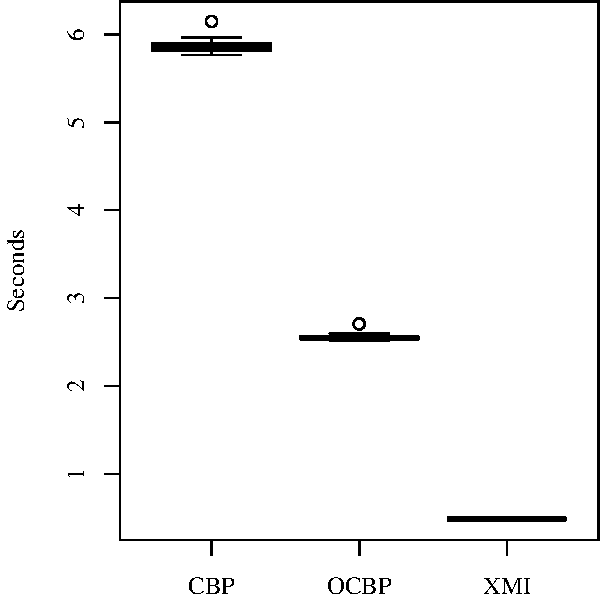
\includegraphics[width=\linewidth]{images/load_time_bpmn2}
        \caption{BPMN2}
        \label{fig:load_time_bpmn2}
    \end{subfigure}
    \hfill
    \begin{subfigure}{0.325\textwidth}
        \centering
        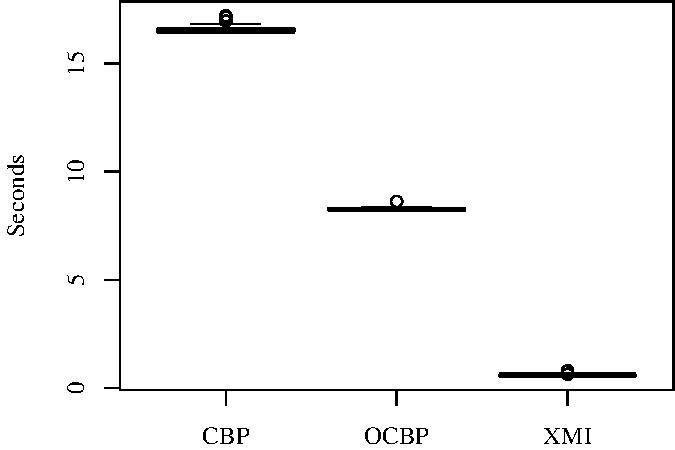
\includegraphics[width=\linewidth]{images/load_time_epsilon}
        \caption{Epsilon}
        \label{fig:load_time_epsilon}
    \end{subfigure}
    \hfill
    \begin{subfigure}{0.325\textwidth}
        \centering
        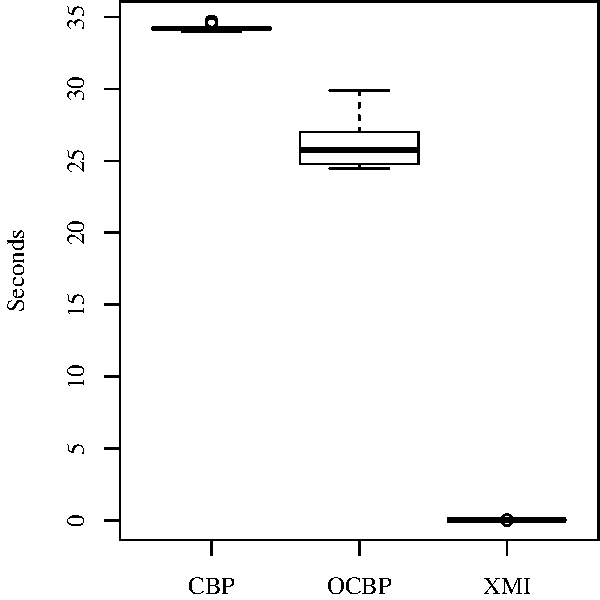
\includegraphics[width=\linewidth]{images/load_time_wikipedia}
        \caption{United States}
        \label{fig:load_time_wikipedia}
    \end{subfigure}
    \caption{A comparison on time required for loading a model between CBP, optimised CBP, and XMI (See Appendix \ref{app:t_test_results} for more detail t-test results).}
    \label{fig:loadtime}
\end{figure}

For this experiment, we then used the proposed and the baseline loading algorithms to reconstruct the state of the three cases' models. The results are shown in Fig. \ref{fig:loadtime} and demonstrate the considerable time savings (up to 56\%, 50\%, and 36\% faster compared to the original CPB implementation of BPMN2, Epsilon, and Unites States cases) delivered by the proposed loading algorithm.

For reference, we also contrast the execution time for the proposed algorithm against that of loading the equivalent state-based model in XMI. As can be observed in Fig. \ref{fig:loadtime}, despite the improvements delivered by the new algorithm, loading change-based models is still outperformed by their state-based counterparts. However, as discussed in\,\cite{yohannis2017turning}, this can be an acceptable trade-off considering the other benefits that change-based model persistence has the potential to offer (e.g. more precise differencing and hence more efficient incremental execution of model management programs and more effective model merging).

\subsection{Saving Time}
\label{subsec:saving_time_test}

\begin{figure}[ht]
    \begin{subfigure}{0.325\textwidth}
        \centering
        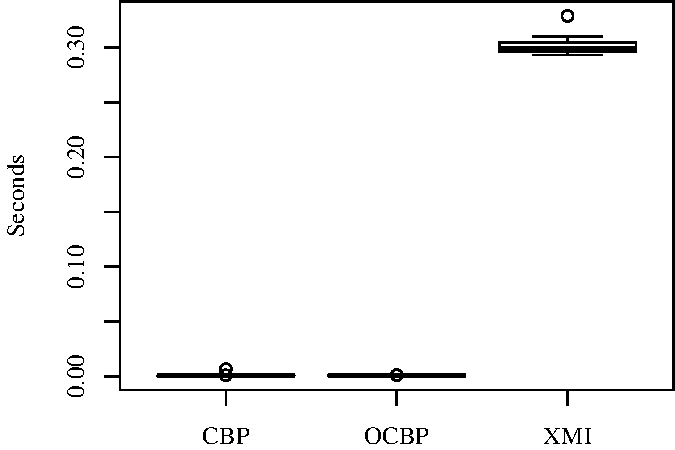
\includegraphics[width=\linewidth]{images/save_time_bpmn2}
        \caption{BPMN2}
        \label{fig:save_time_bpmn2}
    \end{subfigure}
    \hfill
    \begin{subfigure}{0.325\textwidth}
        \centering
        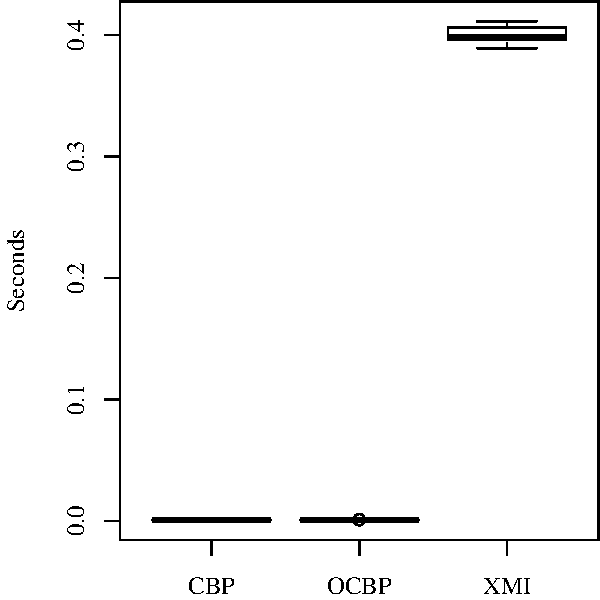
\includegraphics[width=\linewidth]{images/save_time_epsilon}
        \caption{Epsilon}
        \label{fig:save_time_epsilon}
    \end{subfigure}
    \hfill
    \begin{subfigure}{0.325\textwidth}
        \centering
        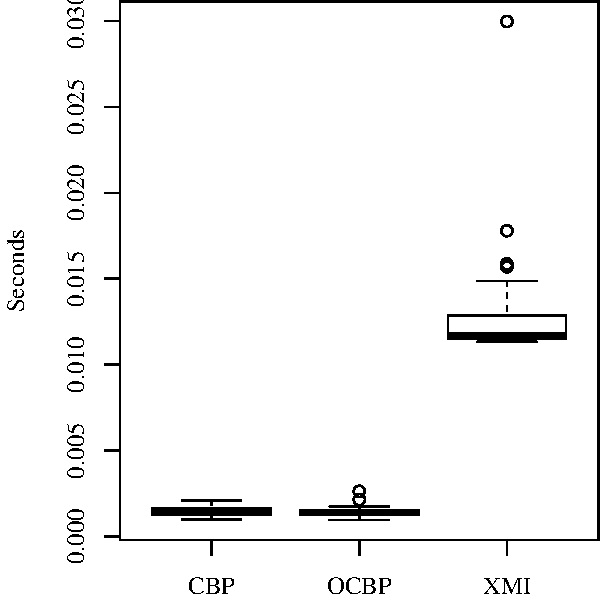
\includegraphics[width=\linewidth]{images/save_time_wikipedia}
        \caption{United States}
        \label{fig:save_time_wikipedia}
    \end{subfigure}
    \caption{A comparison on time required for persisting an event between CBP, optimised CBP, and XMI (See Appendix \ref{app:t_test_results} for more detail t-test results).}
    \label{fig:savetime}
\end{figure}

To achieve the benefits in terms of loading time demonstrated in Section \ref{subsec:loading_time_test}, our algorithm requires additional work to be done (i.e. to assemble the model history data structure and compute the ignore set delta) during the model saving phase as discussed in Section \ref{sec:loading_time_optimisation}. To assess the impact of this additional work on the overall time required to save changes in models, we used the models of the three cases and measure the time required to persist a single change made to a model into a change-based file compared to the time required to persist the whole model in XMI. 

As shown in Fig. \ref{fig:savetime} the performance of the two CBP implementations is almost indistinguishable, which indicates that the cost of the extra work needed by the proposed algorithm at this stage is negligible. On the other hand, CBP implementations are significantly faster at saving changes than XMI. This is expected as the CBP implementations only need to save the last set of changes every time by appending them to the existing model file (and hence their performance is relative to the number of changes since last saved), while the XMI implementation needs to reconstruct an XML document for the entire state of the model and replace the contents of the model file every time (and hence its performance is relative to the size of the entire model). 
         
\subsection{Memory Footprint}
\label{subsec:memory_consumption}

As the proposed loading algorithm requires the maintenance of an additional in-memory data structure that keeps track of element and feature editing histories (see Fig. \ref{fig:history_structure}), we have conducted an additional experiment to measure its memory footprint after loading models and persisting single changes using the models from the three cases. The results are plotted in Fig. \ref{fig:loadmemory} and \ref{fig:savememory}, and demonstrate the significant overhead of the used data structure. We also include the memory footprints of XMI to contrast it with both CBP implementations. As observed, XMI outperforms the optimised CBP representation and performs slightly better than the original CBP representation in terms of its memory footprint when loading models, but is outperformed by both CBP representations when persisting changes. Furthermore, both CBP representations only have a slight difference on time in terms of persisting changes.

\begin{figure}[t]
    \begin{subfigure}{0.325\textwidth}
        \centering
        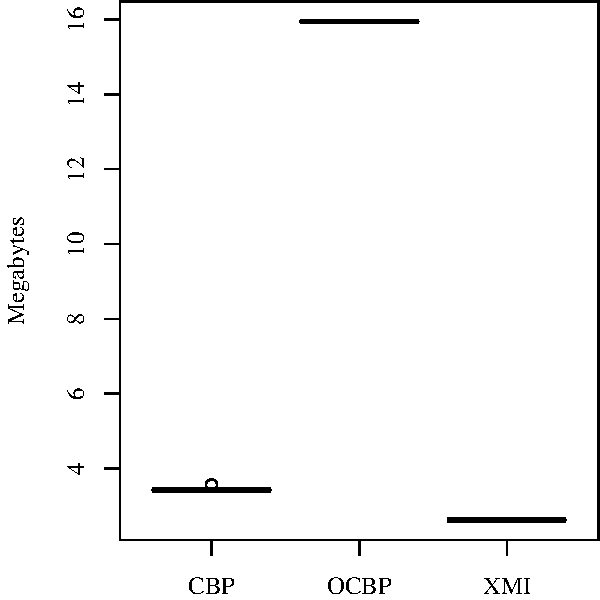
\includegraphics[width=\linewidth]{images/load_memory_bpmn2}
        \caption{BPMN2}
        \label{fig:load_memory_bpmn2}
    \end{subfigure}
    \hfill
    \begin{subfigure}{0.325\textwidth}
        \centering
        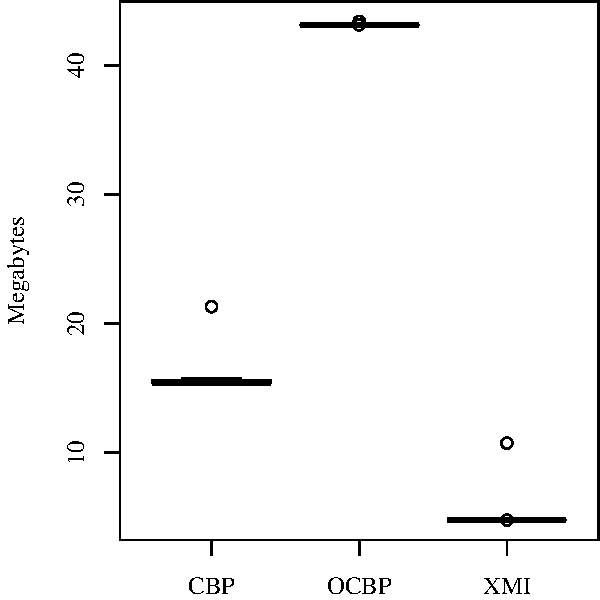
\includegraphics[width=\linewidth]{images/load_memory_epsilon}
        \caption{Epsilon}
        \label{fig:load_memory_epsilon}
    \end{subfigure}
    \hfill
    \begin{subfigure}{0.325\textwidth}
        \centering
        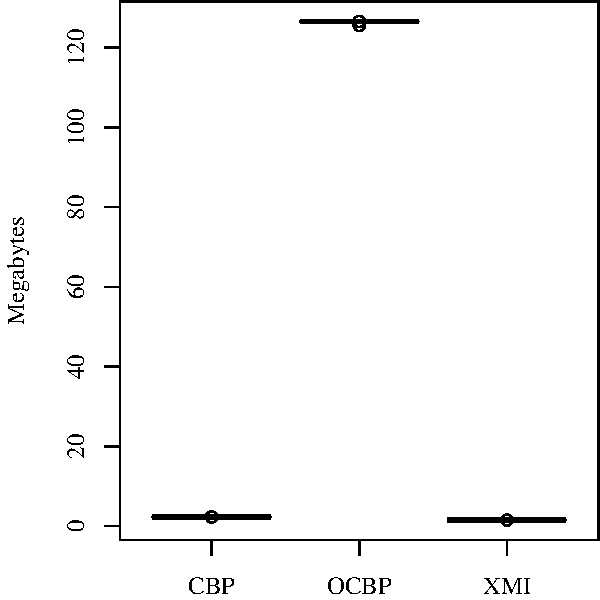
\includegraphics[width=\linewidth]{images/load_memory_wikipedia}
        \caption{United States}
        \label{fig:load_memory_wikipedia}
    \end{subfigure}
    \caption{A comparison on memory footprint after loading a model between CBP, optimised CBP, and XMI (See Appendix \ref{app:t_test_results} for more detail t-test results).}
    \label{fig:loadmemory}
\end{figure}

\begin{figure}[t]
    \begin{subfigure}{0.325\textwidth}
        \centering
        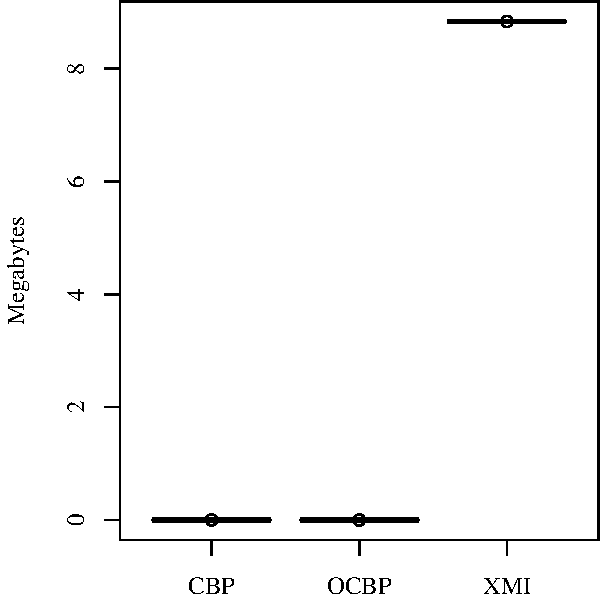
\includegraphics[width=\linewidth]{images/save_memory_bpmn2}
        \caption{BPMN2}
        \label{fig:save_memory_bpmn2}
    \end{subfigure}
    \hfill
    \begin{subfigure}{0.325\textwidth}
        \centering
        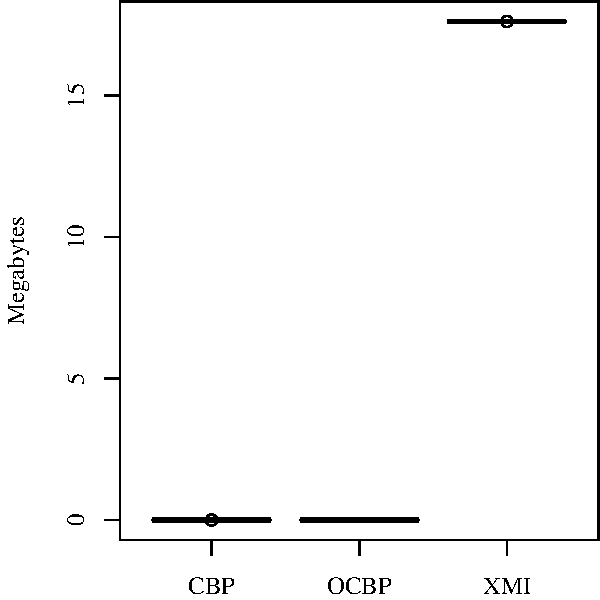
\includegraphics[width=\linewidth]{images/save_memory_epsilon}
        \caption{Epsilon}
        \label{fig:save_memory_epsilon}
    \end{subfigure}
    \hfill
    \begin{subfigure}{0.325\textwidth}
        \centering
        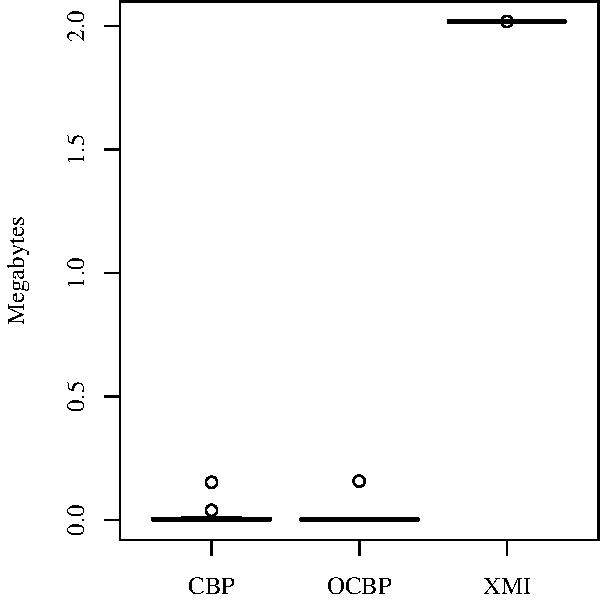
\includegraphics[width=\linewidth]{images/save_memory_wikipedia}
        \caption{United States}
        \label{fig:save_memory_wikipedia}
    \end{subfigure}
    \caption{A comparison on memory footprint after persisting an event between CBP, optimised CBP, and XMI (See Appendix \ref{app:t_test_results} for more detail t-test results).}
    \label{fig:savememory}
\end{figure}



\subsection{Threats to Validity and Limitations}
\label{sec:limitations_and_future_work}
In this work, we have only tested the algorithm on synthesised conference models which may not be representative of the complexity and interconnectedness of models in other domains. Diverse characteristics of models in different domains can affect the effectiveness of the algorithm and therefore yield different outcomes. 

We only support ordered and unique features so far. Support for duplicate values means that removal of an item does not necessarily result in the item not being present in the feature value. Additional information must be captured to persist the number of copies and positions of the feature members to properly generate the ignore set. 

\section{Related Work}
\label{sec:related_work}

Several works have investigated alternative -- but also state-based -- model persistence mechanisms to XMI, mainly by leveraging databases (both relational and NoSQL). For example, EMF Teneo\,\cite{eclipse2017teneo} persists EMF models in relational databases, while Morsa \cite{pagan2011morsa} and NeoEMF \cite{daniel2016neoemf} persist models in document and graph databases respectively. The main challenge with such approaches is version control. None of these approaches provides built-in support for versioning and models are eventually stored in binary files/folders which are known to be a poor fit for text-oriented version control systems like Git and SVN.

Connected Data Objects (CDO) \cite{eclipse2017cdo}, provides support for database-backed model persistence as well as collaboration facilities, but its adoption necessitates the use of a separate version control system in the software development process (e.g. a Git repository for code and a CDO repository for models), which introduces well-recognised fragmentation and administration challenges \cite{barmpis2014evaluation}. Similar challenges are related to the adoption of other model-specific version control systems such as EMFStore\,\cite{koegel2010emfstore}.

\section{Conclusions and Future Work}
\label{sec:conclusions}
In this paper, we have proposed an efficient algorithm and supporting data structures for loading change-based models.
We implemented and evaluated the algorithm on synthesised models against the existing change-based implementation, and state-based XMI. 
Our results show considerable savings in terms of loading time with a negligible impact on saving time, but at the cost of a higher memory footprint.

For future work, we plan to perform experiments in which human modellers will be asked to construct complex models using different modelling languages and persist their change histories. We then plan to scale these up, and evaluate the proposed algorithm against them to assess its impact on real-world models.

Directions for future work include optimising the CBP format so that it consumes less memory and can be parsed faster, and developing a hybrid persistence representation that offers a combination of state-based and change-based persistence. We also plan to investigate the impact of change-based model persistence on change detection, model merging, and conflict resolution of models in the context of collaborative modelling, among others.

%\subsubsection*{Acknowledgments.} This work was partly supported through a scholarship managed by \emph{Lembaga Pengelola Dana Pendidikan Indonesia} (Indonesia Endowment Fund for Education).
%\clearpage
\bibliography{references} 
\bibliographystyle{splncs}

\section*{Appendix: T-test Results}
\label{app:t_test_results}
CBP = Change-based Persistence, OCBP = Optimised CBP, XMI = XML Metadata Interchange, Mean = average, SD = standard deviation, t = ttest t-value, df = degree of freedom, p-value = significance. For time, the unit is seconds. For memory, the unit is Megabytes.

%%%==========================LOAD TIME=======================================
\begin{table}[ht]
\centering
\label{table:ttest_load_time_bpmn2}
\caption{T-test results on loading time for the BPMN2 case.}
\begin{minipage}{0.44\textwidth}
    \centering
        \begin{tabular}{|p{0.20\textwidth}|p{0.34\textwidth}|p{0.36\textwidth}|}
            \hline 
            \textbf{Group}  & \textbf{Mean} & \textbf{SD} \\ 
            \hline 
            \textbf{CBP} & 5.8684750   &0.07871924 \\ 
            \hline 
            \textbf{OCBP} & 2.5553372  & 0.03820040  \\ 
            \hline 
            \textbf{XMI} & 0.4873959   & 0.01062147\\ 
            \hline 
        \end{tabular} 
\end{minipage}
\hfill
\begin{minipage}{0.54\textwidth}
    \centering
    \begin{tabular}{|p{0.38\textwidth}|p{0.2\textwidth}|p{0.2\textwidth}|p{0.22\textwidth}|}
        \hline 
        \textbf{Comparison} & \textbf{t}  & \textbf{df} & \textbf{p-value} \\ 
        \hline 
        \textbf{CBP vs XM}I & 331.88    &23.837 & $<$ 2.2e-16 \\ 
        \hline 
        \textbf{CBP vs OCBP} & 185.5 & 33.263  & $<$ 2.2e-16 \\ 
        \hline 
        \textbf{OCBP vs XMI} & 255.51    & 26.535  & $<$ 2.2e-16 \\ 
        \hline 
    \end{tabular} 
\end{minipage}
\end{table}

\begin{table}[ht]
    \centering
    \label{table:ttest_load_time_epsilon}
    \caption{T-test results on loading time for the Epsilon case.}
    \begin{minipage}{0.44\textwidth}
        \centering
        \begin{tabular}{|p{0.20\textwidth}|p{0.34\textwidth}|p{0.36\textwidth}|}
            \hline 
            \textbf{Group}  & \textbf{Mean} & \textbf{SD} \\ 
            \hline 
            \textbf{CBP} & 8.2072909    & 0.11848822 \\ 
            \hline 
            \textbf{OCBP} &  4.1229173  &  0.05857792 \\ 
            \hline 
            \textbf{XMI} & 0.3786575   & 0.08038106 \\ 
            \hline 
        \end{tabular} 
    \end{minipage}
    \hfill
    \begin{minipage}{0.54\textwidth}
        \centering
     \begin{tabular}{|p{0.38\textwidth}|p{0.2\textwidth}|p{0.2\textwidth}|p{0.22\textwidth}|}
            \hline 
            \textbf{Comparison} & \textbf{t}  & \textbf{df} & \textbf{p-value} \\ 
            \hline 
            \textbf{CBP vs XM}I & 267.86   &40.47 & $<$ 2.2e-16 \\ 
            \hline 
            \textbf{CBP vs OCBP} & 151.38 & 33.609 & $<$ 2.2e-16 \\ 
            \hline 
            \textbf{OCBP vs XMI} & 184.42    &42.055  & $<$ 2.2e-16 \\ 
            \hline 
        \end{tabular} 
    \end{minipage}
\end{table}


\begin{table}[ht]
    \centering
    \label{table:ttest_load_time_wikipedia}
    \caption{T-test results on loading time for the United States case.}
    \begin{minipage}{0.44\textwidth}
        \centering
        \begin{tabular}{|p{0.20\textwidth}|p{0.34\textwidth}|p{0.36\textwidth}|}
            \hline 
            \textbf{Group}  & \textbf{Mean} & \textbf{SD} \\ 
            \hline 
            \textbf{CBP} & 36.42234953     & 2.30316553 \\ 
            \hline 
            \textbf{OCBP} & 23.43390561  &  0.52681953 \\ 
            \hline 
            \textbf{XMI} &  0.02942241  & 0.01680501 \\ 
            \hline 
        \end{tabular} 
    \end{minipage}
    \hfill
    \begin{minipage}{0.54\textwidth}
        \centering
          \begin{tabular}{|p{0.38\textwidth}|p{0.2\textwidth}|p{0.2\textwidth}|p{0.22\textwidth}|}
            \hline 
            \textbf{Comparison} & \textbf{t}  & \textbf{df} & \textbf{p-value} \\ 
            \hline 
            \textbf{CBP vs XM}I &77.408   &23.002 & $<$ 2.2e-16 \\ 
            \hline 
            \textbf{CBP vs OCBP} &  26.932 & 25.4 & $<$ 2.2e-16 \\ 
            \hline 
            \textbf{OCBP vs XMI} & 217.53   & 23.047 & $<$ 2.2e-16 \\ 
            \hline 
        \end{tabular} 
    \end{minipage}
\end{table}

%%%==========================SAVE TIME=======================================
\begin{table}[ht]
    \centering
    \label{table:ttest_save_time_bpmn2}
    \caption{T-test results on saving time for the BPMN2 case.}
    \begin{minipage}{0.44\textwidth}
        \centering
        \begin{tabular}{|p{0.20\textwidth}|p{0.34\textwidth}|p{0.36\textwidth}|}
            \hline 
            \textbf{Group}  & \textbf{Mean} & \textbf{SD} \\ 
            \hline 
            \textbf{CBP} &0.00109375    &0.000498110 \\ 
            \hline 
            \textbf{OCBP} &0.00088420   &0.000052509  \\ 
            \hline 
            \textbf{XMI} & 0.31066177   & 0.006661707 \\ 
            \hline 
        \end{tabular} 
    \end{minipage}
    \hfill
    \begin{minipage}{0.54\textwidth}
        \centering
        \begin{tabular}{|p{0.38\textwidth}|p{0.2\textwidth}|p{0.2\textwidth}|p{0.22\textwidth}|}
            \hline 
            \textbf{Comparison} & \textbf{t}  & \textbf{df} & \textbf{p-value} \\ 
            \hline 
            \textbf{CBP vs XM}I & -227.02    &23.257 & $<$ 2.2e-16 \\ 
            \hline 
            \textbf{CBP vs OCBP} & 2.0496 & 23.511  &0.05171 \\ 
            \hline 
            \textbf{OCBP vs XMI} & -227.8    & 23.003  & $<$ 2.2e-16 \\ 
            \hline 
        \end{tabular} 
    \end{minipage}
\end{table}

\begin{table}[ht]
    \centering
    \label{table:ttest_save_time_epsilon}
    \caption{T-test results on saving time for the Epsilon case.}
    \begin{minipage}{0.44\textwidth}
        \centering
        \begin{tabular}{|p{0.20\textwidth}|p{0.34\textwidth}|p{0.36\textwidth}|}
            \hline 
            \textbf{Group}  & \textbf{Mean} & \textbf{SD} \\ 
            \hline 
            \textbf{CBP} &0.001554733    &  0.0008835900 \\ 
            \hline 
            \textbf{OCBP} &  0.001294067  &  0.0008587366 \\ 
            \hline 
            \textbf{XMI} & 0.249387621   &0.0091627282 \\ 
            \hline 
        \end{tabular} 
    \end{minipage}
    \hfill
    \begin{minipage}{0.54\textwidth}
        \centering
        \begin{tabular}{|p{0.38\textwidth}|p{0.2\textwidth}|p{0.2\textwidth}|p{0.22\textwidth}|}
            \hline 
            \textbf{Comparison} & \textbf{t}  & \textbf{df} & \textbf{p-value} \\ 
            \hline 
            \textbf{CBP vs XM}I & 131.9,    & 23.428 & $<$ 2.2e-16 \\ 
            \hline 
            \textbf{CBP vs OCBP} &1.0364, & 45.963 & 0.3054 \\ 
            \hline 
            \textbf{OCBP vs XMI} & -132.07    &23.404  & $<$ 2.2e-16 \\ 
            \hline 
        \end{tabular} 
    \end{minipage}
\end{table}

\begin{table}[ht]
    \centering
    \label{table:ttest_save_time_wikipedia}
    \caption{T-test results on saving time for the United States case.}
    \begin{minipage}{0.44\textwidth}
        \centering
        \begin{tabular}{|p{0.20\textwidth}|p{0.34\textwidth}|p{0.36\textwidth}|}
            \hline 
            \textbf{Group}  & \textbf{Mean} & \textbf{SD} \\ 
            \hline 
            \textbf{CBP} & 0.001465963     &0.0002902780 \\ 
            \hline 
            \textbf{OCBP} & 0.001451692  &  0.0003469539 \\ 
            \hline 
            \textbf{XMI} & 0.013225421  & 0.0039748169 \\ 
            \hline 
        \end{tabular} 
    \end{minipage}
    \hfill
    \begin{minipage}{0.54\textwidth}
        \centering
        \begin{tabular}{|p{0.38\textwidth}|p{0.2\textwidth}|p{0.2\textwidth}|p{0.22\textwidth}|}
            \hline 
            \textbf{Comparison} & \textbf{t}  & \textbf{df} & \textbf{p-value} \\ 
            \hline 
            \textbf{CBP vs XM}I &-14.455   & 23.245 & $<$ 2.2e-16 \\ 
            \hline 
            \textbf{CBP vs OCBP} &   0.15455 & 44.611 & 0.8779 \\ 
            \hline 
            \textbf{OCBP vs XMI} & -14.456   & 23.35 & $<$ 2.2e-16 \\ 
            \hline 
        \end{tabular} 
    \end{minipage}
\end{table}

%%%==========================LOAD MEMORY=======================================
\begin{table}[ht]
    \centering
    \label{table:ttest_load_memory_bpmn2}
    \caption{T-test results on load memory footprint for the BPMN2 case.}
    \begin{minipage}{0.44\textwidth}
        \centering
        \begin{tabular}{|p{0.20\textwidth}|p{0.34\textwidth}|p{0.36\textwidth}|}
            \hline 
            \textbf{Group}  & \textbf{Mean} & \textbf{SD} \\ 
            \hline 
            \textbf{CBP} & 3.44  & 0.02675 \\ 
            \hline 
            \textbf{OCBP} & 15.94 & 0.000000000  \\ 
            \hline 
            \textbf{XMI} & 2.63   & 0.00045\\ 
            \hline 
        \end{tabular} 
    \end{minipage}
    \hfill
    \begin{minipage}{0.54\textwidth}
        \centering
     \begin{tabular}{|p{0.38\textwidth}|p{0.2\textwidth}|p{0.2\textwidth}|p{0.22\textwidth}|}
            \hline 
            \textbf{Comparison} & \textbf{t}  & \textbf{df} & \textbf{p-value} \\ 
            \hline 
            \textbf{CBP vs XM}I & 148.54  & 23.01 & $<$ 2.2e-16 \\ 
            \hline 
            \textbf{CBP vs OCBP} & -2290.3 & 23 & $<$ 2.2e-16 \\ 
            \hline 
            \textbf{OCBP vs XMI} & 143550   & 23  & $<$ 2.2e-16 \\ 
            \hline 
        \end{tabular} 
    \end{minipage}
\end{table}

\begin{table}[ht]
    \centering
    \label{table:ttest_load_memory_epsilon}
    \caption{T-test results on load memory footprint for the Epsilon case.}
    \begin{minipage}{0.44\textwidth}
        \centering
        \begin{tabular}{|p{0.20\textwidth}|p{0.34\textwidth}|p{0.36\textwidth}|}
            \hline 
            \textbf{Group}  & \textbf{Mean} & \textbf{SD} \\ 
            \hline 
            \textbf{CBP} & 3.143657     &0.0044673582 \\ 
            \hline 
            \textbf{OCBP} & 21.892310  & 0.000000000 \\ 
            \hline 
            \textbf{XMI} & 2.945218   &0.014750126 \\ 
            \hline 
        \end{tabular} 
    \end{minipage}
    \hfill
    \begin{minipage}{0.54\textwidth}
        \centering
        \begin{tabular}{|p{0.38\textwidth}|p{0.2\textwidth}|p{0.2\textwidth}|p{0.22\textwidth}|}
            \hline 
            \textbf{Comparison} & \textbf{t}  & \textbf{df} & \textbf{p-value} \\ 
            \hline 
            \textbf{CBP vs XM}I &63.078  &27.184 & $<$ 2.2e-16 \\ 
            \hline 
            \textbf{CBP vs OCBP} & -20560 & 23 & $<$ 2.2e-16 \\ 
            \hline 
            \textbf{OCBP vs XMI} & 6292.9   &23   & $<$ 2.2e-16 \\ 
            \hline 
        \end{tabular} 
    \end{minipage}
\end{table}


\begin{table}[ht]
    \centering
    \label{table:ttest_load_memory_wikipedia}
    \caption{T-test results on load memory footprint for the United States case.}
    \begin{minipage}{0.44\textwidth}
        \centering
        \begin{tabular}{|p{0.20\textwidth}|p{0.34\textwidth}|p{0.36\textwidth}|}
            \hline 
            \textbf{Group}  & \textbf{Mean} & \textbf{SD} \\ 
            \hline 
            \textbf{CBP} & 2.468129     & 0.4753551354 \\ 
            \hline 
            \textbf{OCBP} & 114.476037  &  0.0015513435 \\ 
            \hline 
            \textbf{XMI} &  1.476961  &  0.0007474206 \\ 
            \hline 
        \end{tabular} 
    \end{minipage}
    \hfill
    \begin{minipage}{0.54\textwidth}
        \centering
        \begin{tabular}{|p{0.38\textwidth}|p{0.2\textwidth}|p{0.2\textwidth}|p{0.22\textwidth}|}
            \hline 
            \textbf{Comparison} & \textbf{t}  & \textbf{df} & \textbf{p-value} \\ 
            \hline 
            \textbf{CBP vs XM}I & 10.215   &23 & $<$ 2.2e-16 \\ 
            \hline 
            \textbf{CBP vs OCBP} & -1154.3, &23 & $<$ 2.2e-16 \\ 
            \hline 
            \textbf{OCBP vs XMI} &321470  &33.132 & $<$ 2.2e-16 \\ 
            \hline 
        \end{tabular} 
    \end{minipage}
\end{table}
   
%%%==========================SAVE MEMORY=======================================
\begin{table}[ht]
    \centering
    \label{table:ttest_save_memory_bpmn2}
    \caption{T-test results on save memory footprint for the BPMN2 case.}
    \begin{minipage}{0.44\textwidth}
        \centering
        \begin{tabular}{|p{0.20\textwidth}|p{0.34\textwidth}|p{0.36\textwidth}|}
            \hline 
            \textbf{Group}  & \textbf{Mean} & \textbf{SD} \\ 
            \hline 
            \textbf{CBP} & 3.220833e-05  & 8.171689e-05 \\ 
            \hline 
            \textbf{OCBP} & 5.874583e-04 & 8.807703e-05  \\ 
            \hline 
            \textbf{XMI} & 8.836976   & 0.000000 \\ 
            \hline 
        \end{tabular} 
    \end{minipage}
    \hfill
    \begin{minipage}{0.54\textwidth}
        \centering
        \begin{tabular}{|p{0.38\textwidth}|p{0.2\textwidth}|p{0.2\textwidth}|p{0.22\textwidth}|}
            \hline 
            \textbf{Comparison} & \textbf{t}  & \textbf{df} & \textbf{p-value} \\ 
            \hline 
            \textbf{CBP vs XM}I & -529780  & 23 & $<$ 2.2e-16 \\ 
            \hline 
            \textbf{CBP vs OCBP} & -22.64 & 45.744 & $<$ 2.2e-16 \\ 
            \hline 
            \textbf{OCBP vs XMI} & -491490   & 23  & $<$ 2.2e-16 \\ 
            \hline 
        \end{tabular} 
    \end{minipage}
\end{table}

\begin{table}[ht]
    \centering
    \label{table:ttest_save_memory_epsilon}
    \caption{T-test results on save memory footprint for the Epsilon case.}
    \begin{minipage}{0.44\textwidth}
        \centering
        \begin{tabular}{|p{0.20\textwidth}|p{0.34\textwidth}|p{0.36\textwidth}|}
            \hline 
            \textbf{Group}  & \textbf{Mean} & \textbf{SD} \\ 
            \hline 
            \textbf{CBP} & 0.000105750      &9.305270e-05 \\ 
            \hline 
            \textbf{OCBP} & 0.000656667   & 7.118846e-05 \\ 
            \hline 
            \textbf{XMI} &8.964714667   & 1.306395e-05 \\ 
            \hline 
        \end{tabular} 
    \end{minipage}
    \hfill
    \begin{minipage}{0.54\textwidth}
        \centering
        \begin{tabular}{|p{0.38\textwidth}|p{0.2\textwidth}|p{0.2\textwidth}|p{0.22\textwidth}|}
            \hline 
            \textbf{Comparison} & \textbf{t}  & \textbf{df} & \textbf{p-value} \\ 
            \hline 
            \textbf{CBP vs XM}I &-467380 &23.906& $<$ 2.2e-16 \\ 
            \hline 
            \textbf{CBP vs OCBP} &-23.036  &43.053 & $<$ 2.2e-16 \\ 
            \hline 
            \textbf{OCBP vs XMI} & -606750 &24.547  & $<$ 2.2e-16 \\ 
            \hline 
        \end{tabular} 
    \end{minipage}
\end{table}


\begin{table}[ht]
    \centering
    \label{table:ttest_save_memory_wikipedia}
    \caption{T-test results on save memory footprint for the United States case.}
    \begin{minipage}{0.44\textwidth}
        \centering
        \begin{tabular}{|p{0.20\textwidth}|p{0.34\textwidth}|p{0.36\textwidth}|}
            \hline 
            \textbf{Group}  & \textbf{Mean} & \textbf{SD} \\ 
            \hline 
            \textbf{CBP} & 0.01031842     & 3.149521e-02 \\ 
            \hline 
            \textbf{OCBP} & 0.00838850  & 3.182750e-02 \\ 
            \hline 
            \textbf{XMI} &  2.01852500  & 1.469694e-05 \\ 
            \hline 
        \end{tabular} 
    \end{minipage}
    \hfill
    \begin{minipage}{0.54\textwidth}
        \centering
        \begin{tabular}{|p{0.38\textwidth}|p{0.2\textwidth}|p{0.2\textwidth}|p{0.22\textwidth}|}
            \hline 
            \textbf{Comparison} & \textbf{t}  & \textbf{df} & \textbf{p-value} \\ 
            \hline 
            \textbf{CBP vs XM}I & -312.37   &23 & $<$ 2.2e-16 \\ 
            \hline 
            \textbf{CBP vs OCBP} &0.21115 &45.995 & $<$ 0.8337 \\ 
            \hline 
            \textbf{OCBP vs XMI} &-309.41  &23 & $<$ 2.2e-16 \\ 
            \hline 
        \end{tabular} 
    \end{minipage}
\end{table}
\end{document} 
               